\documentclass[11pt]{article}
\usepackage{amsmath,amsthm,amsfonts,amssymb, xcolor,enumerate,enumitem,xfrac,tikz,comment, pgfplots,soul, mathtools, minted, fontspec, standalone}
\usetikzlibrary{shapes.geometric,positioning,calc}
\usepackage{url}
\usepackage[colorlinks=true,
            linkcolor=blue,
            filecolor=magenta,
            urlcolor=black,
            citecolor=magenta,
            pdftitle={Reviewing report},
            pdfpagemode=FullScreen,
          ]{hyperref}

\newcommand{\R}{\mathbb{R}}
\newcommand{\Norm}[1]{\left|\left|  #1   \right|\right|}
\newcommand{\E}{\mathbb{E}}
\newcommand{\ud}{\ensuremath{\mathrm{d}}}

\setmonofont{DejaVu Sans Mono}[Scale=MatchLowercase]

\newcommand{\FoxH}[5]{H_{#2}^{#1}\left(#3\:\middle\vert\: \begin{array}{l}#4\\[0.4em] #5\end{array}\right)}
\newcommand{\FoxHext}[7]{
  \renewcommand{\arraystretch}{1.5} % Adjust the factor 1.5 as needed
  H_{#2}^{#1}\left(#3\:\middle\vert\:
  \begin{array}{c|c}
    #4 & #5 \\ \hline
    #6 & #
  \end{array}
  \right)
}
\renewcommand{\arraystretch}{1.8}

\begin{document}

\title{Some symbolic tools for the {F}ox {$H$}-function}
\author{Le Chen                             \\
  Department of Maathematics and Statistics \\
  Auburn University                         \\
\url{le.chen@auburn.edu}, \url{chenle02@gmail.com}
}

\maketitle

In this note, we explain the code for checking the conditions of the Fox
$H$-function~\cite{fox:61:g}. Here we follow the notation from Kilbas and
Saigo~\cite{kilbas.saigo:04:h-transforms}. \bigskip


Let $m,n,p,q$ be configure integers such that
\begin{align*}
  0 \le m \le q \quad \text{and} \quad
  0 \le n \le p.
\end{align*}
Let $a_i,b_j\in \mathbb{C}$ and $\alpha_i, \beta_j \in\R_+$ be the parameters given below:
\begin{center}
\renewcommand{\arraystretch}{1.2}
  \begin{tabular}{|c|cc|c|}
    \hline
    $\in \left(\mathbb{C},\R_+\right)$ & Front list                              & Rear list                                       &            \\ \hline
    $p$                                & $(a_1,\alpha_1),\cdots, (a_n,\alpha_n)$ & $(a_{n+1},\alpha_{n+1}),\cdots, (a_p,\alpha_p)$ & Upper list \\
    $q$                                & $(b_1,\beta_1),\cdots, (b_m,\beta_m)$   & $(b_{m+1},\beta_{m+1}),\cdots, (b_q,\beta_q)$   & Lower list \\ \hline
  \end{tabular}
\end{center}
and denote
\begin{align}\label{E:H}
  \mathcal{H}^{m,n}_{p,q}(s) \coloneqq
         \dfrac{ \displaystyle \prod_{i=1}^n\Gamma\left(1-a_i-\alpha_is\right) }{ \displaystyle \prod_{i=n+1}^p\Gamma\left(a_j+\alpha_is\right)    }
  \times \dfrac{ \displaystyle \prod_{j=1}^m\Gamma\left(b_j+\beta_js\right)    }{ \displaystyle \prod_{j=m+1}^q\Gamma\left(1- b_j-\alpha_js\right) }\:.
\end{align}
Then the Fox $H$-function $\FoxH{2,1}{2,3}{z}{\cdots}{\cdots}$ is defined by a Mellin-Barnes type integral of the form
\begin{align}\label{E:Fox-H}
  \FoxH{p,q}{m,n}{z}{(a_1,\alpha_1),\cdots, (a_p,\alpha_p)}{(b_1,\beta_1),\cdots, (b_q,\beta_q)}
  \coloneqq \frac{1}{2\pi i} \int_{\mathcal{L}} H^{m,n}_{p,q}(s) z^{-s} \ud s.
\end{align}

The basic assumption for the well-posedness of the Fox H-function is that two
sets of poles do not overlap, i.e.,
\begin{align}\label{E:poles}
  \bigg\{b_{j\ell}=\frac{-b_j-\ell}{\beta_j },  \ell =0, 1, \cdots\bigg\} \bigcap
  \bigg\{a_{ik}   =\frac{1-a_i + k}{\alpha_i},  k=0, 1,     \cdots\bigg\} = \emptyset.
\end{align}

The contour $\mathcal{L}$ in~\eqref{E:Fox-H} is given by one of the following
three cases:
\begin{enumerate}

  \item $\mathcal{L}=\mathcal{L}_{-\infty}$ is a left loop situated in a
    horizontal strip starting at point $-\infty+i\phi_1$ and terminating at
    point $-\infty+i\phi_2$ for some $-\infty<\phi_1< \phi_2<\infty$;

  \item $\mathcal{L}=\mathcal{L}_{+\infty}$ is a right loop situated in a
    horizontal strip starting at point $+\infty+i\phi_1$ and terminating at
    point $\infty+i\phi_2$ for some $-\infty<\phi_1< \phi_2<\infty$;

  \item $\mathcal{L}=\mathcal{L}_{i\gamma\infty}$ is a contour starting at point
    $\gamma-i\infty$ and terminating at point $\gamma+i\infty$ for some
    $\gamma\in(-\infty, \infty)$.

\end{enumerate}

We need a set of conditions to ensure the convergence of the integral
in~\eqref{E:Fox-H}. To explain this, we need to introduce some notation
(following~p.~2~of~\cite{kilbas.saigo:04:h-transforms}). First denote
\begin{align*}
  a_1^* & \coloneqq \sum_{j=1}^{m}\beta_j  - \sum_{i=n+1}^{p}\alpha_i, \\
  a_2^* & \coloneqq \sum_{i=1}^{n}\alpha_i - \sum_{j=m+1}^{q}\beta_j .
\end{align*}
The following two parameters play the most important role:
\begin{alignat*}{4}
  a^*    & \coloneqq a^*_2 + a^*_1 &  & =  \sum_{i=1}^n \alpha_i -\sum_{i=n+1}^p \alpha_i + \sum_{j=1}^m \beta_j - \sum_{j=m+1}^{q}\beta_j; \\
  \Delta & \coloneqq a^*_2 - a^*_1 &  & = \sum_{j=1}^q\beta_j-\sum_{i=1}^p\alpha_i.
\end{alignat*}
Similar to $a^*$, we define
\begin{align*}
  \xi & \coloneqq \sum_{i=1}^n a_i -\sum_{i=n+1}^p a_i + \sum_{j=1}^m b_j - \sum_{j=m+1}^{q} b_j.
\end{align*}
Additionally, set
\begin{align*}
  c^* \coloneqq m+n - \frac{p+q}{2}.
\end{align*}
In the critical cases, we need to use the following two parameters:
\begin{align*}
  \delta & \coloneqq \prod_{i=1}^{p}\alpha_i^{-\alpha_i} \prod_{j=1}^{q}\beta_j^{\beta_i}; \\
  \mu    & \coloneqq \sum_{j=1}^{q}b_j - \sum_{i=1}^{p}a_i + \frac{p-q}{2}                 \\
\end{align*}

\begin{figure}[htp]
  \centering
  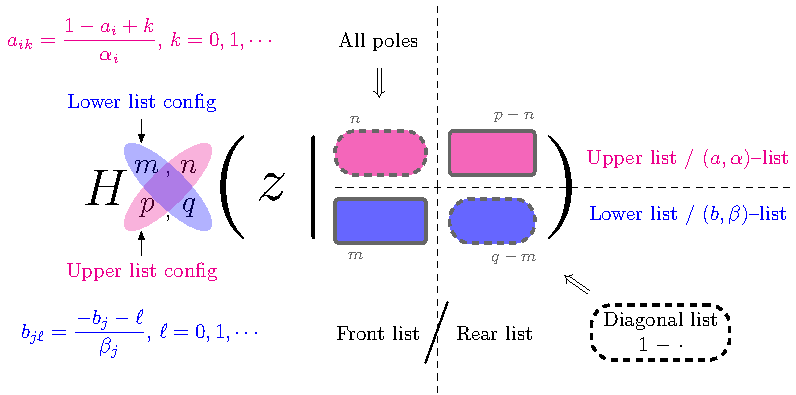
\includegraphics[width=1.0\textwidth]{./FoxH-Diagram.pdf}
  \caption{Diagram for the parameterization of the Fox $H$-function.}
  \label{F:Diagram}
\end{figure}

The well-posedness of the Fox $H$-function is given by Theorems 1.1 and 1.2
of~\cite{kilbas.saigo:04:h-transforms}, which are summarized in the following
figure~\ref{F:Wellposedness}:

\begin{figure}[htp]
  \centering
  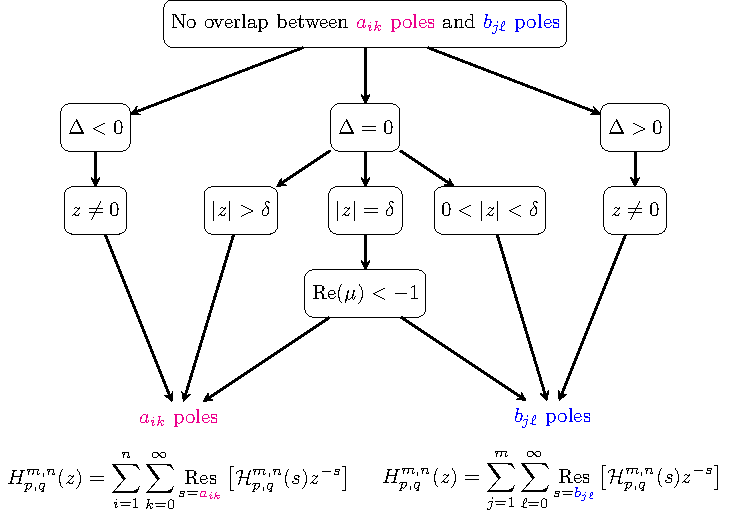
\includegraphics[width=1.0\textwidth]{./Well-posedness.pdf}
  \caption{Well-posedness of the Fox $H$-function.}
  \label{F:Wellposedness}
\end{figure}

\documentclass{article}
\usepackage{amsmath, url, hyperref, minted, fontspec}
\setmonofont{DejaVu Sans Mono}[Scale=MatchLowercase]
\newcommand{\FoxH}[5]{H_{#2}^{#1}\left(#3\:\middle\vert\: \begin{array}{l}#4\\[0.4em] #5\end{array}\right)}
\newcommand{\FoxHext}[7]{
  \renewcommand{\arraystretch}{1.5} % Adjust the factor 1.5 as needed
  H_{#2}^{#1}\left(#3\:\middle\vert\:
  \begin{array}{c|c}
    #4 & #5 \\ \hline
    #6 & #7
  \end{array}
  \right)
}
\renewcommand{\arraystretch}{1.8}

\begin{document}

\section{Example \url{FoxH32-21.wls}}

\paragraph{File content}

\inputminted{text}{FoxH32-21.wls}

\paragraph{Fox H-function}

\begin{align*}
  \FoxH
    {2,1}
    {2,3}
    {\cdot}
    {\left(1, \frac{1}{\alpha }\right), \left(\text{Ceil}(\beta ), \beta\right)}
    {\left(\frac{1}{2}, \frac{\alpha }{2}\right), \left(1, 1\right), \left(1, \frac{\alpha }{2}\right)}
\end{align*}

\begin{align*}
  \FoxHext
    {2,1}
    {2,3}
    {\cdot}
    {\left(1, \frac{1}{\alpha }\right)}
    {\left(\text{Ceil}(\beta ), \beta\right)}
    {\left(\frac{1}{2}, \frac{\alpha }{2}\right), \left(1, 1\right)}
    {\left(1, \frac{\alpha }{2}\right)}
\end{align*}

\paragraph{Summary}

\begin{align*}
  a^*    & = \frac{1}{\alpha }-\beta +1 \\
  \Delta & = \alpha -\frac{1}{\alpha }-\beta +1 \\
  \delta & = 2^{-\alpha } \left(\frac{1}{\alpha }\right)^{-1/\alpha } \left(2^{\alpha /2} \alpha ^{\alpha /2}+\alpha ^{\alpha }\right) \beta ^{-\beta } \\
  \mu    & = 1-\text{Ceil}(\beta ) \\
  a_1^*  & = \frac{1}{2} (\alpha -2 \beta +2) \\
  a_2^*  & = \frac{1}{\alpha }-\frac{\alpha }{2} \\
  \xi    & = \frac{3}{2}-\text{Ceil}(\beta ) \\
  c^*    & = \frac{1}{2} \\
\end{align*}

\paragraph{Poles}

\noindent\textbf{1. First ten poles from upper front list}

\begin{align*}
  a_{i,k} = 
  \left(
\begin{array}{c}
 0 \\
 \alpha  \\
 2 \alpha  \\
 3 \alpha  \\
 4 \alpha  \\
 5 \alpha  \\
 6 \alpha  \\
 7 \alpha  \\
 8 \alpha  \\
 9 \alpha  \\
 10 \alpha  \\
\end{array}
\right)
\end{align*}
\noindent\textbf{2. First ten poles from lower front list}

\begin{align*}
  b_{j,\ell} = 
  \left(
\begin{array}{cc}
 -\frac{1}{\alpha } & -1 \\
 -\frac{3}{\alpha } & -2 \\
 -\frac{5}{\alpha } & -3 \\
 -\frac{7}{\alpha } & -4 \\
 -\frac{9}{\alpha } & -5 \\
 -\frac{11}{\alpha } & -6 \\
 -\frac{13}{\alpha } & -7 \\
 -\frac{15}{\alpha } & -8 \\
 -\frac{17}{\alpha } & -9 \\
 -\frac{19}{\alpha } & -10 \\
 -\frac{21}{\alpha } & -11 \\
\end{array}
\right)
\end{align*}

\end{document}
\documentclass[11pt]{article}


\usepackage{amsmath, url, hyperref, minted, fontspec}
\setmonofont{DejaVu Sans Mono}[Scale=MatchLowercase]
\newcommand{\FoxH}[5]{H_{#2}^{#1}\left(#3\:\middle\vert\: \begin{array}{l}#4\\[0.4em] #5\end{array}\right)}
\newcommand{\FoxHext}[7]{
  \renewcommand{\arraystretch}{1.5} % Adjust the factor 1.5 as needed
  H_{#2}^{#1}\left(#3\:\middle\vert\:
  \begin{array}{c|c}
    #4 & #5 \\ \hline
    #6 & #7
  \end{array}
  \right)
}
\renewcommand{\arraystretch}{1.8}

% -------------------------------------------------
% BibTex Setup
% -------------------------------------------------
\usepackage[strict=true,style=english]{csquotes}
\setlength{\parskip}{0.5cm plus4mm minus3mm}
\usepackage[
  backend=biber,
  style=alphabetic,
  natbib=true,
  abbreviate=true
  ]{biblatex}

\addbibresource{../latex_sources/Fox-H_biber.bib}
\begin{document}

\section{Example \url{FoxH32-21-Y.wls}}

\paragraph{File content}

\inputminted{text}{FoxH32-21-Y.wls}

\paragraph{Fox H-function}

\begin{align*}
  \FoxH
    {2,1}
    {2,3}
    {\cdot}
    {\left(1, 1\right), \left(\beta +\gamma, \beta\right)}
    {\left(\frac{d}{2}, \frac{\alpha }{2}\right), \left(1, 1\right), \left(1, \frac{\alpha }{2}\right)}
\end{align*}

\begin{align*}
  \FoxHext
    {2,1}
    {2,3}
    {\cdot}
    {\left(1, 1\right)}
    {\left(\beta +\gamma, \beta\right)}
    {\left(\frac{d}{2}, \frac{\alpha }{2}\right), \left(1, 1\right)}
    {\left(1, \frac{\alpha }{2}\right)}
\end{align*}

\paragraph{Summary}

\begin{align*}
  a^*    & = 2-\beta \\
  \Delta & = \alpha -\beta \\
  \delta & = 2^{-\alpha } \left(2^{\alpha /2} \alpha ^{\alpha /2}+\alpha ^{\alpha }\right) \beta ^{-\beta } \\
  \mu    & = \frac{1}{2} (-2 \beta -2 \gamma +d+1) \\
  a_1^*  & = \frac{1}{2} (\alpha -2 \beta +2) \\
  a_2^*  & = 1-\frac{\alpha }{2} \\
  \xi    & = \frac{1}{2} (d-2 (\beta +\gamma -1)) \\
  c^*    & = \frac{1}{2} \\
\end{align*}

\paragraph{Poles}

\noindent\textbf{1. First eight poles from upper front list}

\begin{align*}
  a_{i,k} = 
  \left(
\begin{array}{cccccccc}
 0 & 1 & 2 & 3 & 4 & 5 & 6 & 7 \\
\end{array}
\right)
\end{align*}
\noindent\textbf{2. First eight poles from lower front list}

\begin{align*}
  b_{j,\ell} = 
  \left(
\begin{array}{cccccccc}
 -\frac{d}{\alpha } & -\frac{d+2}{\alpha } & -\frac{d+4}{\alpha } & -\frac{d+6}{\alpha } & -\frac{d+8}{\alpha } & -\frac{d+10}{\alpha } & -\frac{d+12}{\alpha } & -\frac{d+14}{\alpha } \\
 -1 & -2 & -3 & -4 & -5 & -6 & -7 & -8 \\
\end{array}
\right)
\end{align*}

\printbibliography[title={References}]

\end{document}
\documentclass[11pt]{article}


\usepackage{amsmath, url, hyperref, minted, fontspec}
\setmonofont{DejaVu Sans Mono}[Scale=MatchLowercase]
\newcommand{\FoxH}[5]{H_{#2}^{#1}\left(#3\:\middle\vert\: \begin{array}{l}#4\\[0.4em] #5\end{array}\right)}
\newcommand{\FoxHext}[7]{
  \renewcommand{\arraystretch}{1.5} % Adjust the factor 1.5 as needed
  H_{#2}^{#1}\left(#3\:\middle\vert\:
  \begin{array}{c|c}
    #4 & #5 \\ \hline
    #6 & #7
  \end{array}
  \right)
}
\renewcommand{\arraystretch}{1.8}

% -------------------------------------------------
% BibTex Setup
% -------------------------------------------------
\usepackage[strict=true,style=english]{csquotes}
\setlength{\parskip}{0.5cm plus4mm minus3mm}
\usepackage[
  backend=biber,
  style=alphabetic,
  natbib=true,
  abbreviate=true
  ]{biblatex}

\addbibresource{../latex_sources/Fox-H_biber.bib}
\begin{document}

\section{Example \url{FoxH32-21-Z.wls}}

\paragraph{File content}

\inputminted{text}{FoxH32-21-Z.wls}

\paragraph{Fox H-function}

\begin{align*}
  \FoxH
    {2,1}
    {2,3}
    {\cdot}
    {\left(1, 1\right), \left(\lceil \beta \rceil, \beta\right)}
    {\left(\frac{d}{2}, \frac{\alpha }{2}\right), \left(1, 1\right), \left(1, \frac{\alpha }{2}\right)}
\end{align*}

\begin{align*}
  \FoxHext
    {2,1}
    {2,3}
    {\cdot}
    {\left(1, 1\right)}
    {\left(\lceil \beta \rceil, \beta\right)}
    {\left(\frac{d}{2}, \frac{\alpha }{2}\right), \left(1, 1\right)}
    {\left(1, \frac{\alpha }{2}\right)}
\end{align*}

\paragraph{Summary}

\begin{align*}
  a^*    & = 2-\beta \\
  \Delta & = \alpha -\beta \\
  \delta & = 2^{-\alpha } \left(2^{\alpha /2} \alpha ^{\alpha /2}+\alpha ^{\alpha }\right) \beta ^{-\beta } \\
  \mu    & = \frac{1}{2} (-2 \lceil \beta \rceil +d+1) \\
  a_1^*  & = \frac{1}{2} (\alpha -2 \beta +2) \\
  a_2^*  & = 1-\frac{\alpha }{2} \\
  \xi    & = \frac{1}{2} (-2 \lceil \beta \rceil +d+2) \\
  c^*    & = \frac{1}{2} \\
\end{align*}

\paragraph{Poles}

\noindent\textbf{1. First eight poles from upper front list}

\begin{align*}
  a_{i,k} = 
  \left(
\begin{array}{cccccccc}
 0 & 1 & 2 & 3 & 4 & 5 & 6 & 7 \\
\end{array}
\right)
\end{align*}
\noindent\textbf{2. First eight poles from lower front list}

\begin{align*}
  b_{j,\ell} = 
  \left(
\begin{array}{cccccccc}
 -\frac{d}{\alpha } & -\frac{d+2}{\alpha } & -\frac{d+4}{\alpha } & -\frac{d+6}{\alpha } & -\frac{d+8}{\alpha } & -\frac{d+10}{\alpha } & -\frac{d+12}{\alpha } & -\frac{d+14}{\alpha } \\
 -1 & -2 & -3 & -4 & -5 & -6 & -7 & -8 \\
\end{array}
\right)
\end{align*}


% \addbibresource{../latex_sources/Fox-H_biber.bib}

\paragraph{Source} This is the fundamental solution to the fractional diffusion
equation used, e.g., in~\cite{chen.hu.ea:17:space-time, chen.hu.ea:19:nonlinear,
chen.eisenberg:22:interpolating, chen.guo.ea:22:moments}.


\printbibliography[title={References}]

\end{document}
\documentclass{article}
\usepackage{amsmath}
\newcommand{\FoxH}[5]{H_{#2}^{#1}\left(#3\:\middle\vert\: \begin{subarray}{l}#4\\[0.4em] #5\end{subarray}\right)}
\begin{document}
\begin{align*}
\FoxH{2,3}{2,1}{\cdot}{\left(1, 1\right), \left(1, \beta\right)}{\left(\frac{d}{2}, \frac{\alpha }{2}\right), \left(1, 1\right), \left(1, \frac{\alpha }{2}\right)}
\end{align*}
\noindent\textbf{Summary}
\begin{align*}
a^* &= 2-\beta \\
\Delta &= \alpha -\beta \\
\delta &= 2^{-\alpha } \left(2^{\alpha /2} \alpha ^{\alpha /2}+\alpha ^{\alpha }\right) \beta ^{-\beta } \\
\mu &= \frac{d-1}{2} \\
a_1^* &= \frac{1}{2} (\alpha -2 \beta +2) \\
a_2^* &= 1-\frac{\alpha }{2} \\
\xi &= \frac{d}{2} \\
c^* &= \frac{1}{2} \\
\end{align*}
\end{document}
\documentclass[11pt]{article}


\usepackage{amsmath, url, hyperref, minted, fontspec}
\setmonofont{DejaVu Sans Mono}[Scale=MatchLowercase]
\newcommand{\FoxH}[5]{H_{#2}^{#1}\left(#3\:\middle\vert\: \begin{array}{l}#4\\[0.4em] #5\end{array}\right)}
\newcommand{\FoxHext}[7]{
  \renewcommand{\arraystretch}{1.5} % Adjust the factor 1.5 as needed
  H_{#2}^{#1}\left(#3\:\middle\vert\:
  \begin{array}{c|c}
    #4 & #5 \\ \hline
    #6 & #7
  \end{array}
  \right)
}
\renewcommand{\arraystretch}{1.8}

% -------------------------------------------------
% BibTex Setup
% -------------------------------------------------
\usepackage[strict=true,style=english]{csquotes}
\setlength{\parskip}{0.5cm plus4mm minus3mm}
\usepackage[
  backend=biber,
  style=alphabetic,
  natbib=true,
  abbreviate=true
  ]{biblatex}

\addbibresource{../latex_sources/Fox-H_biber.bib}
\begin{document}

\section{Example \url{FoxH-Cos.wls}}

\paragraph{File content}

\inputminted{text}{FoxH-Cos.wls}

\paragraph{Fox H-function}

\begin{align*}
  \FoxH
    {1,0}
    {0,2}
    {\cdot}
    {}
    {\left(0, 1\right), \left(\frac{1}{2}, 1\right)}
\end{align*}

\begin{align*}
  \FoxHext
    {1,0}
    {0,2}
    {\cdot}
    {}
    {}
    {\left(0, 1\right)}
    {\left(\frac{1}{2}, 1\right)}
\end{align*}

\paragraph{Summary}

\begin{align*}
  a^*    & = 0 \\
  \Delta & = 2 \\
  \delta & = \text{ComplexInfinity} \\
  \mu    & = -\frac{1}{2} \\
  a_1^*  & = 1 \\
  a_2^*  & = -1 \\
  \xi    & = -\frac{1}{2} \\
  c^*    & = 0 \\
\end{align*}

\paragraph{Poles}

\noindent\textbf{1. First eight poles from upper front list}

\begin{align*}
  a_{i,k} = 
  \{\}
\end{align*}
\noindent\textbf{2. First eight poles from lower front list}

\begin{align*}
  b_{j,\ell} = 
  \left(
\begin{array}{cccccccc}
 0 & -1 & -2 & -3 & -4 & -5 & -6 & -7 \\
\end{array}
\right)
\end{align*}

\printbibliography[title={References}]

\end{document}
\documentclass[11pt]{article}
\usepackage{amsmath, url, hyperref, minted, fontspec}
\setmonofont{DejaVu Sans Mono}[Scale=MatchLowercase]
\newcommand{\FoxH}[5]{H_{#2}^{#1}\left(#3\:\middle\vert\: \begin{array}{l}#4\\[0.4em] #5\end{array}\right)}


\usepackage{amsmath, url, hyperref, minted, fontspec}
\setmonofont{DejaVu Sans Mono}[Scale=MatchLowercase]
\newcommand{\FoxH}[5]{H_{#2}^{#1}\left(#3\:\middle\vert\: \begin{array}{l}#4\\[0.4em] #5\end{array}\right)}
\newcommand{\FoxHext}[7]{
  \renewcommand{\arraystretch}{1.5} % Adjust the factor 1.5 as needed
  H_{#2}^{#1}\left(#3\:\middle\vert\:
  \begin{array}{c|c}
    #4 & #5 \\ \hline
    #6 & #7
  \end{array}
  \right)
}
\renewcommand{\arraystretch}{1.8}

% -------------------------------------------------
% BibTex Setup
% -------------------------------------------------
\usepackage[strict=true,style=english]{csquotes}
\setlength{\parskip}{0.5cm plus4mm minus3mm}
\usepackage[
  backend=biber,
  style=alphabetic,
  natbib=true,
  abbreviate=true
  ]{biblatex}

\addbibresource{../latex_sources/Fox-H_biber.bib}
\begin{document}

\section{Example \url{FoxH-Mittag-Leffler.wls}}

\paragraph{File content}

\inputminted{text}{FoxH-Mittag-Leffler.wls}

\paragraph{Fox H-function}

\begin{align*}
  \FoxH
    {1,1}
    {1,2}
    {\cdot}
    {\left(0, 1\right)}
    {\left(0, 1\right), \left(1-\mu, \rho\right)}
\end{align*}

\begin{align*}
  \FoxHext
    {1,1}
    {1,2}
    {\cdot}
    {\left(0, 1\right)}
    {}
    {\left(0, 1\right)}
    {\left(1-\mu, \rho\right)}
\end{align*}

\paragraph{Summary}

\begin{align*}
  a^*    & = 2-\rho \\
  \Delta & = \rho \\
  \delta & = \text{ComplexInfinity} \\
  \mu    & = \frac{1}{2}-\mu \\
  a_1^*  & = 1 \\
  a_2^*  & = 1-\rho \\
  \xi    & = \mu -1 \\
  c^*    & = \frac{1}{2} \\
\end{align*}

\paragraph{Poles}

\noindent\textbf{1. First eight poles from upper front list}

\begin{align*}
  a_{i,k} = 
  \left(
\begin{array}{cccccccc}
 1 & 2 & 3 & 4 & 5 & 6 & 7 & 8 \\
\end{array}
\right)
\end{align*}
\noindent\textbf{2. First eight poles from lower front list}

\begin{align*}
  b_{j,\ell} = 
  \left(
\begin{array}{cccccccc}
 0 & -1 & -2 & -3 & -4 & -5 & -6 & -7 \\
\end{array}
\right)
\end{align*}

\printbibliography[title={References}]

\end{document}
\documentclass[preview]{standalone}
\usepackage{amsmath, url, hyperref, minted, fontspec}
\setmonofont{DejaVu Sans Mono}[Scale=MatchLowercase]
\newcommand{\FoxH}[5]{H_{#2}^{#1}\left(#3\:\middle\vert\: \begin{array}{l}#4\\[0.4em] #5\end{array}\right)}
\newcommand{\FoxHext}[7]{
  \renewcommand{\arraystretch}{1.5} % Adjust the factor 1.5 as needed
  H_{#2}^{#1}\left(#3\:\middle\vert\:
  \begin{array}{c|c}
    #4 & #5 \\ \hline
    #6 & #7
  \end{array}
  \right)
}
\renewcommand{\arraystretch}{1.8}

\begin{document}

\section{Example \url{FoxH-Sin.wls}}

\paragraph{File content}

\inputminted{text}{FoxH-Sin.wls}

\paragraph{Fox H-function}

\begin{align*}
  \FoxH
    {1,0}
    {0,2}
    {\cdot}
    {}
    {\left(\frac{1}{2}, 1\right), \left(0, 1\right)}
\end{align*}

\begin{align*}
  \FoxHext
    {1,0}
    {0,2}
    {\cdot}
    {}
    {}
    {\left(\frac{1}{2}, 1\right)}
    {\left(0, 1\right)}
\end{align*}

\paragraph{Summary}

\begin{align*}
  a^*    & = 0 \\
  \Delta & = 2 \\
  \delta & = \text{ComplexInfinity} \\
  \mu    & = -\frac{1}{2} \\
  a_1^*  & = 1 \\
  a_2^*  & = -1 \\
  \xi    & = \frac{1}{2} \\
  c^*    & = 0 \\
\end{align*}

\paragraph{Poles}

\noindent\textbf{1. First ten poles from upper front list}

\begin{align*}
  a_{i,k} = 
  \{\{\},\{\},\{\},\{\},\{\},\{\},\{\},\{\},\{\},\{\},\{\}\}
\end{align*}
\noindent\textbf{2. First ten poles from lower front list}

\begin{align*}
  b_{j,\ell} = 
  \left(
\begin{array}{c}
 -\frac{1}{2} \\
 -\frac{3}{2} \\
 -\frac{5}{2} \\
 -\frac{7}{2} \\
 -\frac{9}{2} \\
 -\frac{11}{2} \\
 -\frac{13}{2} \\
 -\frac{15}{2} \\
 -\frac{17}{2} \\
 -\frac{19}{2} \\
 -\frac{21}{2} \\
\end{array}
\right)
\end{align*}

\end{document}

\bibliographystyle{alpha} \bibliography{../refs/refs.bib}
\end{document}

